\documentclass{beamer}
\mode<presentation>
\usepackage{amsmath,amssymb,mathtools}
\usepackage{textcomp}
\usepackage{gensymb}
\usepackage{adjustbox}
\usepackage{subcaption}
\usepackage{enumitem}
\usepackage{multicol}
\usepackage{listings}
\usepackage{url}
\usepackage{graphicx} % <-- needed for images
\def\UrlBreaks{\do\/\do-}

\usetheme{Boadilla}
\usecolortheme{lily}
\setbeamertemplate{footline}{
  \leavevmode%
  \hbox{%
  \begin{beamercolorbox}[wd=\paperwidth,ht=2ex,dp=1ex,right]{author in head/foot}%
    \insertframenumber{} / \inserttotalframenumber\hspace*{2ex}
  \end{beamercolorbox}}%
  \vskip0pt%
}
\setbeamertemplate{navigation symbols}{}

\lstset{
  frame=single,
  breaklines=true,
  columns=fullflexible,
  basicstyle=\ttfamily\tiny   % tiny font so code fits
}

\numberwithin{equation}{section}

% ---- your macros ----
\providecommand{\nCr}[2]{\,^{#1}C_{#2}}
\providecommand{\nPr}[2]{\,^{#1}P_{#2}}
\providecommand{\mbf}{\mathbf}
\providecommand{\pr}[1]{\ensuremath{\Pr\left(#1\right)}}
\providecommand{\qfunc}[1]{\ensuremath{Q\left(#1\right)}}
\providecommand{\sbrak}[1]{\ensuremath{{}\left[#1\right]}}
\providecommand{\lsbrak}[1]{\ensuremath{{}\left[#1\right.}}
\providecommand{\rsbrak}[1]{\ensuremath{\left.#1\right]}}
\providecommand{\brak}[1]{\ensuremath{\left(#1\right)}}
\providecommand{\lbrak}[1]{\ensuremath{\left(#1\right.}}
\providecommand{\rbrak}[1]{\ensuremath{\left.#1\right)}}
\providecommand{\cbrak}[1]{\ensuremath{\left\{#1\right\}}}
\providecommand{\lcbrak}[1]{\ensuremath{\left\{#1\right.}}
\providecommand{\rcbrak}[1]{\ensuremath{\left.#1\right\}}}
\theoremstyle{remark}
\newtheorem{rem}{Remark}
\newcommand{\sgn}{\mathop{\mathrm{sgn}}}
\providecommand{\abs}[1]{\left\vert#1\right\vert}
\providecommand{\res}[1]{\Res\displaylimits_{#1}}
\providecommand{\norm}[1]{\lVert#1\rVert}
\providecommand{\mtx}[1]{\mathbf{#1}}
\providecommand{\mean}[1]{E\left[ #1 \right]}
\providecommand{\fourier}{\overset{\mathcal{F}}{ \rightleftharpoons}}
\providecommand{\system}{\overset{\mathcal{H}}{ \longleftrightarrow}}
\providecommand{\dec}[2]{\ensuremath{\overset{#1}{\underset{#2}{\gtrless}}}}
\newcommand{\myvec}[1]{\ensuremath{\begin{pmatrix}#1\end{pmatrix}}}
\let\vec\mathbf
% ---------------------

\title{Matgeo Presentation - Problem 1.6.6}
\author{ee25btech11056 - Suraj.N}

\begin{document}

\begin{frame}
  \titlepage
\end{frame}

% Problem Statement
\begin{frame}{Problem Statement}

 In each of the following, find the value of $k$ for which the points are collinear:
  
    (a) $(7,-2),\ (5,1),\ (3,k)$ \\
    (b) $(8,1),\ (k,-4),\ (2,-5)$
  

\end{frame}

% Method
\begin{frame}{Method}
\textbf{Condition for Collinearity:}

Three points $A, B, C$ are collinear iff the collinearity matrix

\begin{align*}
M=\myvec{ \vec{B}-\vec{A} & \vec{C}-\vec{A} }^\top
\end{align*}

has $rank\brak{M}=1$.

\end{frame}

% Part (a)
\begin{frame}{Part (a) Matrix}

\begin{align*}
\myvec{ \vec{B}-\vec{A} & \vec{C}-\vec{A} }^\top = \myvec{-2 & 3\\ -4 & k+2}
\end{align*}

\begin{align*}
\myvec{-2 & 3\\ -4 & k+2}
&\xleftrightarrow{R_2 = R_2 - 2R_1}
\myvec{-2 & 3\\ 0 & k-4}
\end{align*}

For collinearity, $rank\brak{M}=1 \iff k-4=0 \implies \boxed{k=4}$.

\end{frame}

% Part (b)
\begin{frame}{Part (b) Matrix}

\begin{align*}
\myvec{ \vec{B}-\vec{A} & \vec{C}-\vec{A} }^\top = \myvec{k-8 & -5\\ -6 & -6}
\end{align*}

\begin{align*}
\myvec{k-8 & -5\\ -6 & -6}
&\xleftrightarrow{R_2 = (k-8)R_2 + 6R_1}
\myvec{k-8 & -5\\[2pt] 0 & 18-6k}
\end{align*}
For collinearity, $rank\brak{M}=1 \iff 18-6k=0 \implies \boxed{k=3}$.

\end{frame}

\begin{frame}{Final Answer}

 (a) $k=4$ \\
 (b) $k=3$

\end{frame}

% Plots
\begin{frame}{Plots}

\begin{figure}[h!]
\centering
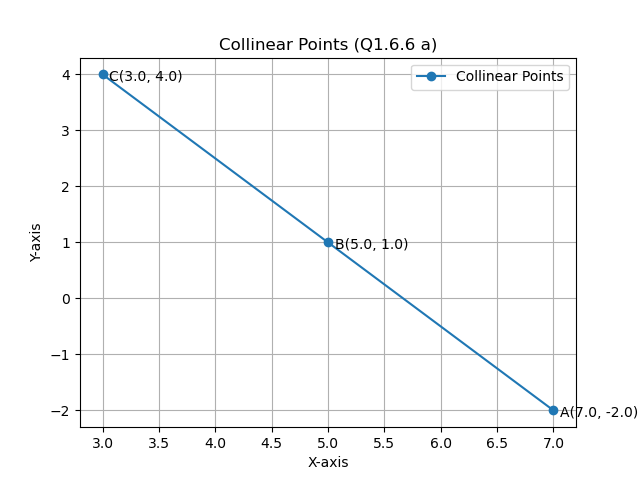
\includegraphics[width=0.7\textwidth]{figs/fig_a.png}\hfill
\caption*{Fig 1 : Line through the given points}
\label{Fig 1}
\end{figure}

\end{frame}

\begin{frame}{Plots}

\begin{figure}[h!]
 \centering
  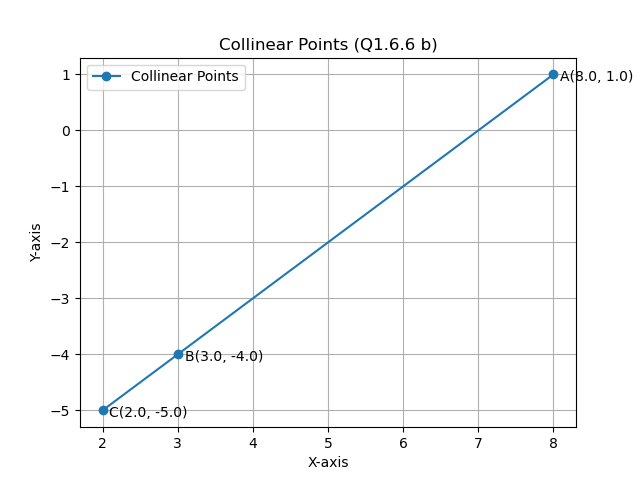
\includegraphics[width=0.7\textwidth]{figs/fig_b.png}
  \caption*{Fig 2 : Line through the given points}
  \label{Fig 2}
\end{figure}

\end{frame}

% --------- CODE APPENDIX ---------
\section*{Appendix: Code}

% C program
\begin{frame}[fragile]{C Code: points.c (Part 1)}
\begin{lstlisting}[language=C]
#include <stdio.h>

int main() {
  FILE *fp;

  // Question 1.6.6 (a)
  int k_a = 4; // Final answer
  printf("Q1.6.6 (a): k = %d\n", k_a);

  fp = fopen("points_a.dat", "w");
  fprintf(fp, "%d,%d,%d\n", 7, -2, 0);  // A
  fprintf(fp, "%d,%d,%d\n", 5, 1, 0);   // B
  fprintf(fp, "%d,%d,%d\n", 3, k_a, 0); // C
  fclose(fp);
\end{lstlisting}
\end{frame}

\begin{frame}[fragile]{C Code: points.c (Part 2)}
\begin{lstlisting}[language=C]
  // Question 1.6.6 (b)
  int k_b = 3; // Final answer
  printf("Q1.6.6 (b): k = %d\n", k_b);

  fp = fopen("points_b.dat", "w");
  fprintf(fp, "%d,%d,%d\n", 8, 1, 0);    // A
  fprintf(fp, "%d,%d,%d\n", k_b, -4, 0); // B
  fprintf(fp, "%d,%d,%d\n", 2, -5, 0);   // C
  fclose(fp);

  return 0;
}
\end{lstlisting}
\end{frame}

% Python calling C
\begin{frame}[fragile]{Python: call\_c.py}
\begin{lstlisting}[language=Python]
import subprocess

# Compile the C program
subprocess.run(["gcc", "points.c", "-o", "points"], check=True)

# Run the compiled C program
result = subprocess.run(
    ["./points"], capture_output=True, text=True, check=True
)

# Print the output from the C program
print(result.stdout)
\end{lstlisting}
\end{frame}

% Python plotting
\begin{frame}[fragile]{Python: plot.py (Part 1)}
\begin{lstlisting}[language=Python]
import numpy as np
import matplotlib.pyplot as plt

def plot_points(filename, labels, title, output_file):
    points = np.loadtxt(filename, delimiter=',', usecols=(0,1))
    x = points[:,0]
    y = points[:,1]

    plt.plot(x, y, 'o-', label='Collinear Points')

    for i, txt in enumerate(labels):
        plt.annotate(f"{txt}{tuple(points[i])}", (x[i], y[i]),
                     xytext=(5,-5), textcoords="offset points")
\end{lstlisting}
\end{frame}

\begin{frame}[fragile]{Python: plot.py (Part 2)}
\begin{lstlisting}[language=Python]
    plt.xlabel("X-axis")
    plt.ylabel("Y-axis")
    plt.title(title)
    plt.legend()
    plt.grid(True)

    plt.savefig(output_file)
    print(f"Saved figure as {output_file}")
    plt.close()

# Part (a)
plot_points("points_a.dat", ["A","B","C"],
            "Collinear Points (Q1.6.6 a)", "fig_a.png")

# Part (b)
plot_points("points_b.dat", ["A","B","C"],
            "Collinear Points (Q1.6.6 b)", "fig_b.png")
\end{lstlisting}
\end{frame}

\end{document}

